\documentclass[10pt,a4paper]{article}
\usepackage[latin1]{inputenc}
\usepackage{amsmath}
\usepackage{amsfonts}
\usepackage{amssymb}
\usepackage{amsthm}
\usepackage{graphicx}
\usepackage[ruled,vlined]{algorithm2e}
\usepackage{hyperref}

\newtheorem{theorem}{Theorem}
\newtheorem{claim}[theorem]{Claim}

\title{Sample Document in \LaTeX}
\author{Your name \\  {\tt Roll no}}
\date{}


%%%%%%%%%%%%%%%%%%%%%%%%%%%%%%%%%%%%%%%%%%%%%%%%%
% Preamble ends before begin{document}

\begin{document}
\maketitle


\section{Sample section}
How much wood would wood chuck chuck if wood chuck would chuck wood ?


\section{Writing Math}
Here we will see how to write math. Normal math symbols : 
$\alpha\beta\gamma\epsilon\phi\Phi $.
\begin{enumerate}
\item Bad math : B=A2+B*ci, B $=$ A $+$ B $*$ c$_i$, phi:A -> N
\item Good math : $B=A^2 +B \times c_{ij}$, $\phi: A \to N$.
\end{enumerate}


\subsection{Writing equations}
\begin{itemize}
\item Normal equations : 
	$\int_0^\infty e^{-x} x^{n-1} \mathrm{d}x = \Gamma(n)$.
\item Display math equation : 
	\begin{equation}
	\int_0^\infty e^{-x} x^{n-1} \mathrm{d}x = \Gamma(n)
	\end{equation}
\item Display math equation with no numbering : 
	\begin{equation*}
	\int_0^\infty e^{-x} x^{n-1} \mathrm{d}x = \Gamma(n)
	\end{equation*}
\item Writing sets
	\begin{equation}
	HP = \left \{ \langle M,x \rangle ~|~ \text{$M$ on inputs $x$ halts}  \right \}
	\end{equation}
	\begin{equation}
	S =  \left \{ i ~\left |  \prod_{d | i} i \text{ is even }, i > 0 \right . \right \}
	\end{equation}
\end{itemize}

\subsection{Aligning equations, writing text in math mode}
\begin{align*}
\sum_{i=1}^n i & = \sum_{i=1}^{n-1} i + n \\
			   & = \frac{(n-1)\cdot n}{2} + n && [\text{By induction hypothesis}]\\
			   & = \frac{n(n+1)}{2}
\end{align*}

\section{Writing Algorithms}
\begin{algorithm}
        \KwResult{Checks if $G$ has an odd cycle of length $k$}
        Set $t \gets \sum_{r=0}^k \begin{bmatrix} k \\ r \end{bmatrix}_2$ \;
        Do something
        \For{$u \in V$}{
                \If{Some condition}{ 
                        Do this \;
                        Do that \;
                }\If{$j > t$}{
                        Reject
                }
        }
        Accept iff all conditions ok
        \caption{Algorithm detecting odd cycle of length $k$}
\end{algorithm}
\begin{itemize}
\item Step 1  :
\item Step 2 :
\end{itemize}


\section{Drawing tables}
\begin{center}
\begin{tabular}{||c|l|l||}
\hline 
\textbf{Type} & \textbf{Language} & \textbf{Machine} \\ 
\hline \hline
Type 3 & Regular & Finite Automata \\ 
\hline 
Type 2 & Context Free & Push Down Automata \\ 
\hline 
Type 1 & Context Sensitive & Linear Bounded Automata \\ 
\hline
Type 0 & Recursively Enumerable & Turing Machine \\ 
\hline 
\end{tabular} 
\end{center}

\section{Writing Theorems and Proofs} \label{sec:rel}
\begin{claim} \label{cl:relativity}
If $m$ is mass and $c$ is speed of light then, 
\begin{equation} \label{eq:relativity}
E = mc^2
\end{equation}

\end{claim}
\begin{proof}
Trivial. 
\end{proof}

\begin{claim} 
There exists  undecidable languages
\end{claim}
\begin{proof}(Idea)
Set of languages is $\mathcal{P}(\Sigma^*)$ is uncountably infinite,
while set of all Turing machines which can be identified with 
$\Sigma^*$ is only countably infinite. 

\end{proof}
\begin{theorem}
A language is decidable if and only if its complement is also decidable.
\end{theorem}

\begin{proof}
($\Longrightarrow$) Forward direction

($\Longleftarrow$) Reverse direction

\end{proof}



\section{Referring sections and theorems}
Recalling equation~\ref{eq:relativity} in claim~\ref{cl:relativity} from section~\ref{sec:rel},
it is possible to generate energy from nuclear reactions.


\section{Including Images}

\begin{figure}[htp!]
\centering
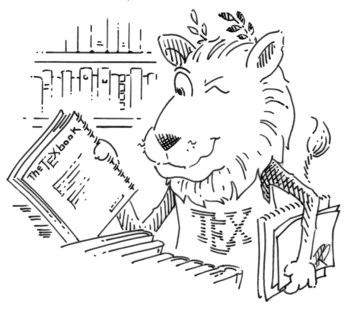
\includegraphics[scale=0.7]{tex-lion}
\caption{CTAN lion (or lioness ?) drawing by Duane Bibby}
\end{figure}


\section{Compilation}


\end{document}
